\chapter{Planning}

In the table~\ref{tab:plan} the planning for the project can be observed. The workloads can be seen
in the table~\ref{tab:work}. It has been decided to do Task 3 and Task 4 in parallel even if that
supposes to divide the working day in two tasks, since having only one resource and being part of
the development of the same intermediate product, both tasks could benefit from the parallel
development. The same decision has been made with tasks T14 and T15 for the same reasons.

\begin{table}[h]
	\centering
	\caption{Project planning.}\label{tab:plan}
	\begin{tabular}{ccccccc}
		\toprule
		\textbf{Task} & \emph{Dep.} & \emph{Resource} & \emph{Days} & \emph{Work} & \emph{Start date} & \emph{Ending date}\\
		\midrule
		T1	&				& Project Manager		& 1 day		&	2 hours		& 01/07/2015	& 01/07/2015	\\
		T2	&				& Project Manager		& 1 day		&	2 hours		& 01/07/2015	& 01/07/2015	\\
		T3	&	T1			& Programmer			& 8 days	&	32 hours	& 01/08/2015	& 01/19/2015	\\
		T4	&	T2			& Designer				& 8 days	&	16 hours	& 01/26/2015	& 02/04/2015	\\
		T5	&	T3			& Programmer			& 18 days	&	56 hours	& 01/20/2015	& 01/16/2015	\\
		T6	&	T4			& Designer				& 7 days	&	28 hours	& 02/17/2015	& 02/25/2015	\\
		T7	&	T5, T6		& WebLab-Deusto	Expert	& 8 days	&	32 hours	& 02/26/2015	& 03/09/2015	\\
		T8	&	T7			& Project Manager		& 1 day		&	2 hours		& 03/13/2015	& 03/13/2015	\\
		T9	&	T8			& Programmer			& 2 days	&	8 hours		& 03/16/2015	& 03/17/2015	\\
		T10	&	T9			& Programmer			& 8 days	&	32 hours	& 03/18/2015	& 03/31/2015	\\
		T11	&	T10			& WebLab-Deusto	Expert	& 4 days	&	16 hours	& 04/13/2015	& 04/16/2015	\\
		T12	&	T11			& Project Manager		& 2 days	&	8 hours		& 04/17/2015	& 04/20/2015	\\
		T13	&	T12			& Programmer			& 5 days	&	20 hours	& 04/21/2015	& 04/27/2015	\\
		T14	&	T13			& Programmer			& 9 days	&	20 hours	& 04/28/2015	& 05/11/2015	\\
		T15	&	T12			& Designer				& 8 days	&	16 hours	& 04/28/2015	& 05/08/2015	\\
		T16	&	T14, T15	& WebLab-Deusto	Expert	& 12 days	&	48 hours	& 05/12/2015	& 05/27/2015	\\
		T17	&	T7			& Project Manager		& 3 days	&	12 hours	& 03/10/2015	& 03/12/2015	\\
		\bottomrule
	\end{tabular}
\end{table}

\begin{table}[h]
	\centering
	\caption{Project workloads.}\label{tab:work}
	\begin{tabular}{cc}
		\toprule
		\textbf{Profile} & \emph{Scheduled hours} \\
		\midrule
		Project Manager			&	26 hours	\\
		Programmer				&	168 hours	\\
		Designer				&	60 hours	\\
		WebLab-Deusto Expert	&	96 hours	\\
		\bottomrule
	\end{tabular}
\end{table}

The Gantt diagram of the project can be seen in figure~\ref{fig:gantt} and the precedence diagram in
figure~\ref{fig:precedence}.

% Gantt diagram in four pages
\clearpage
\begin{figure}
	\centering
	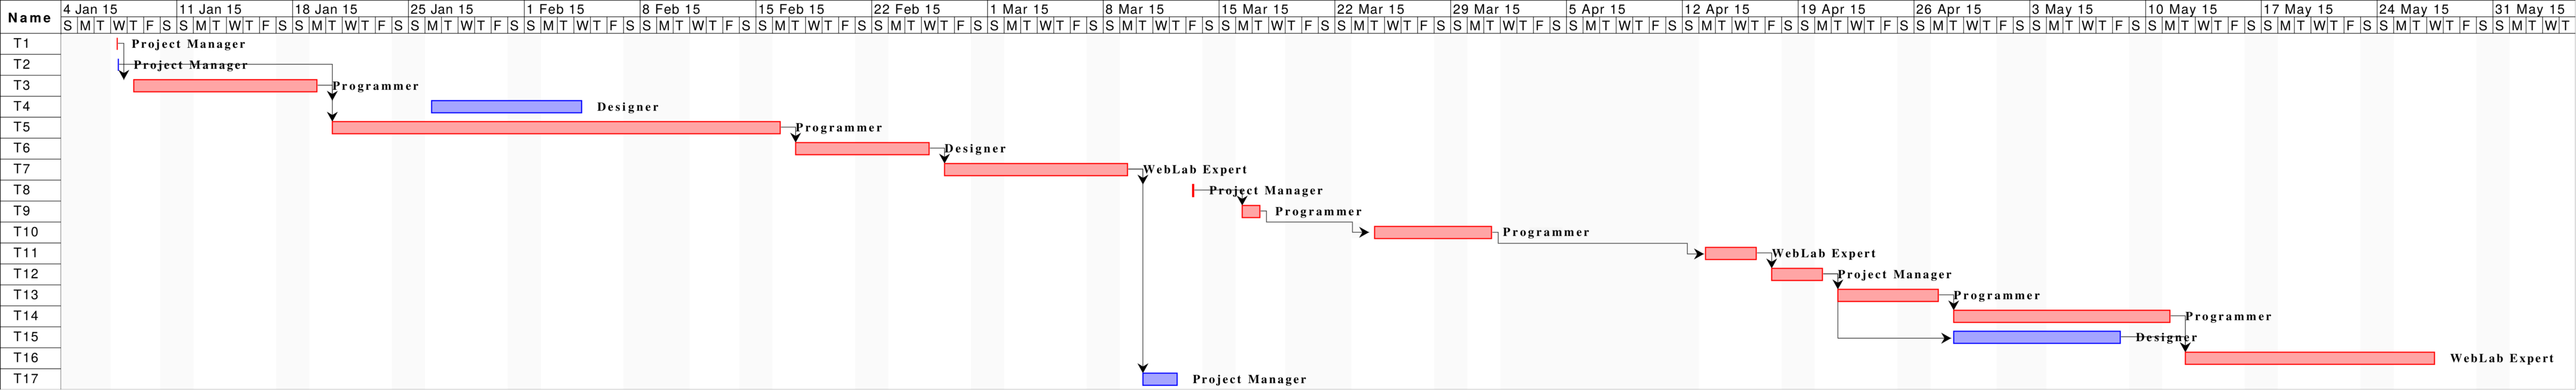
\includegraphics[trim=0in 0in 26in 0in, clip, angle=90]{fig/gantt}
	\caption[Gantt diagram of the project.]{Gantt diagram of the project. Continues in next
	pages.}\label{fig:gantt}
\end{figure}
\clearpage

\begin{center}
	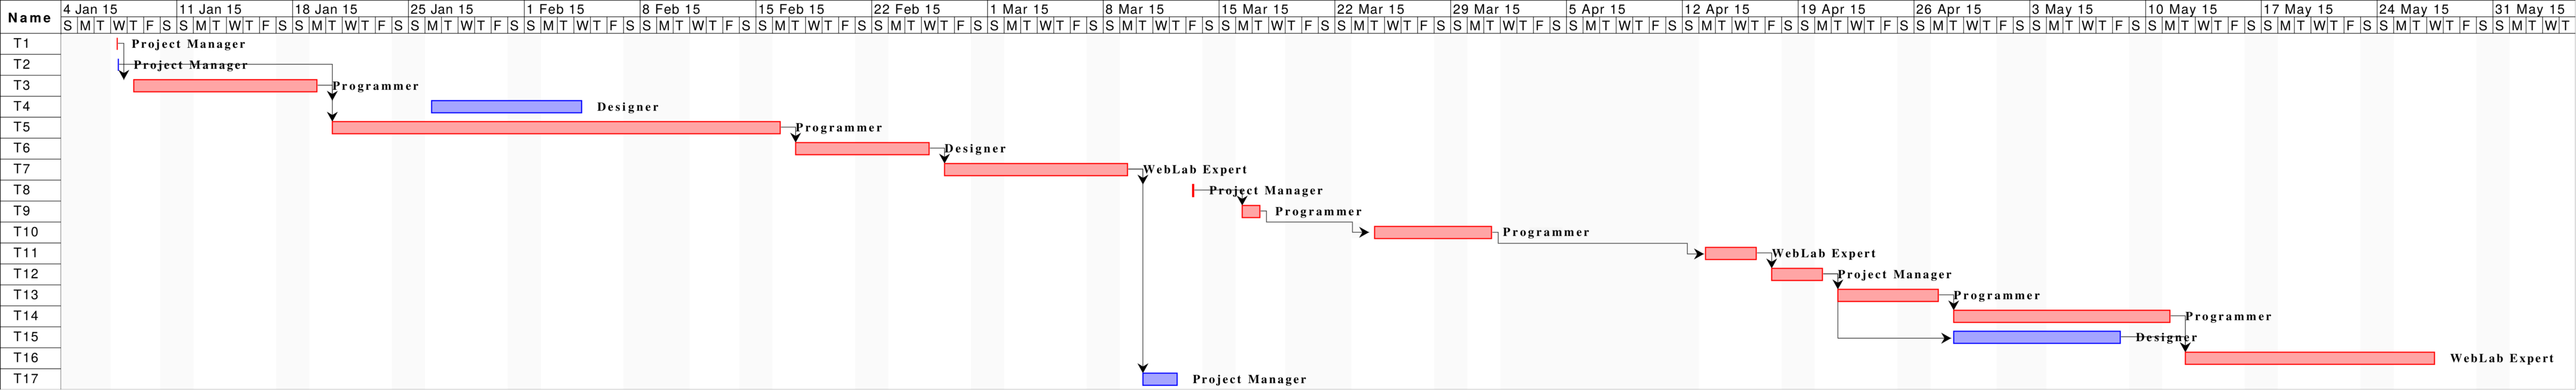
\includegraphics[trim=7.82in 0in 17in 0in, clip, angle=90]{fig/gantt}
	\clearpage

	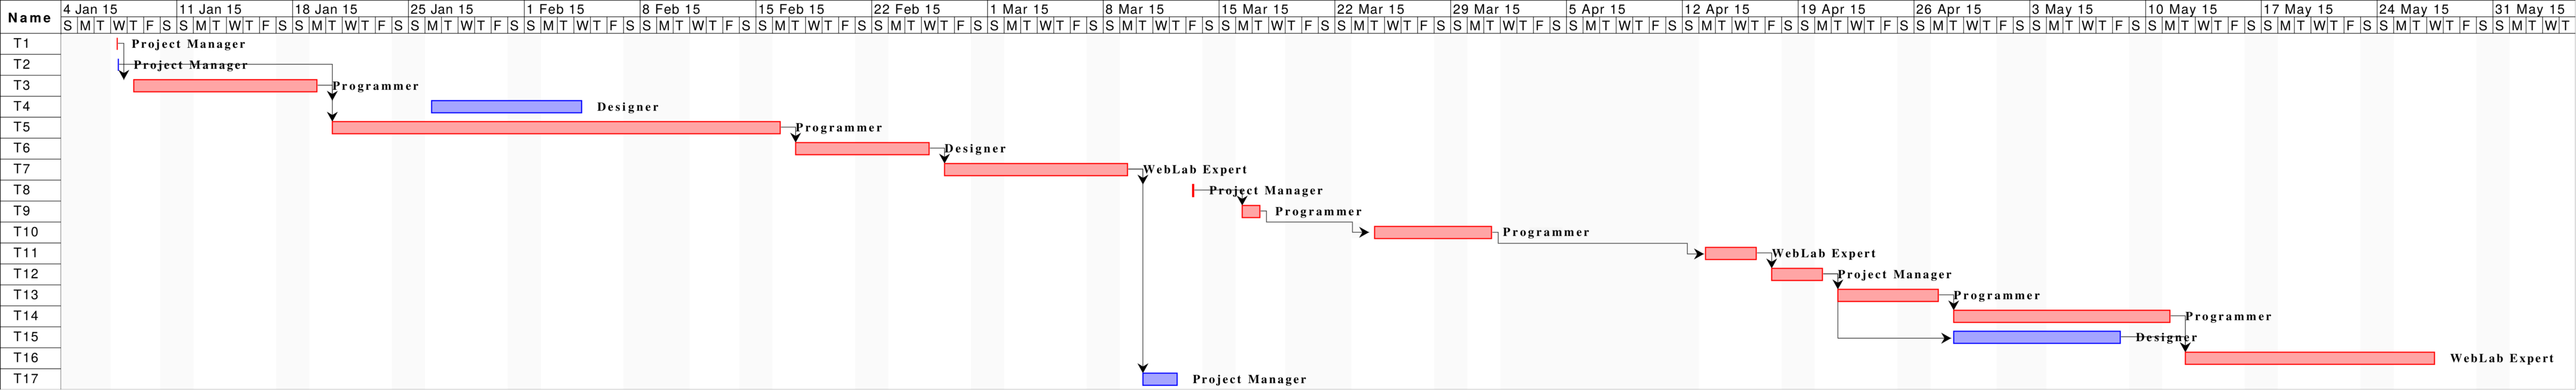
\includegraphics[trim=16.82in 0in 8in 0in, clip, angle=90]{fig/gantt}
	\clearpage

	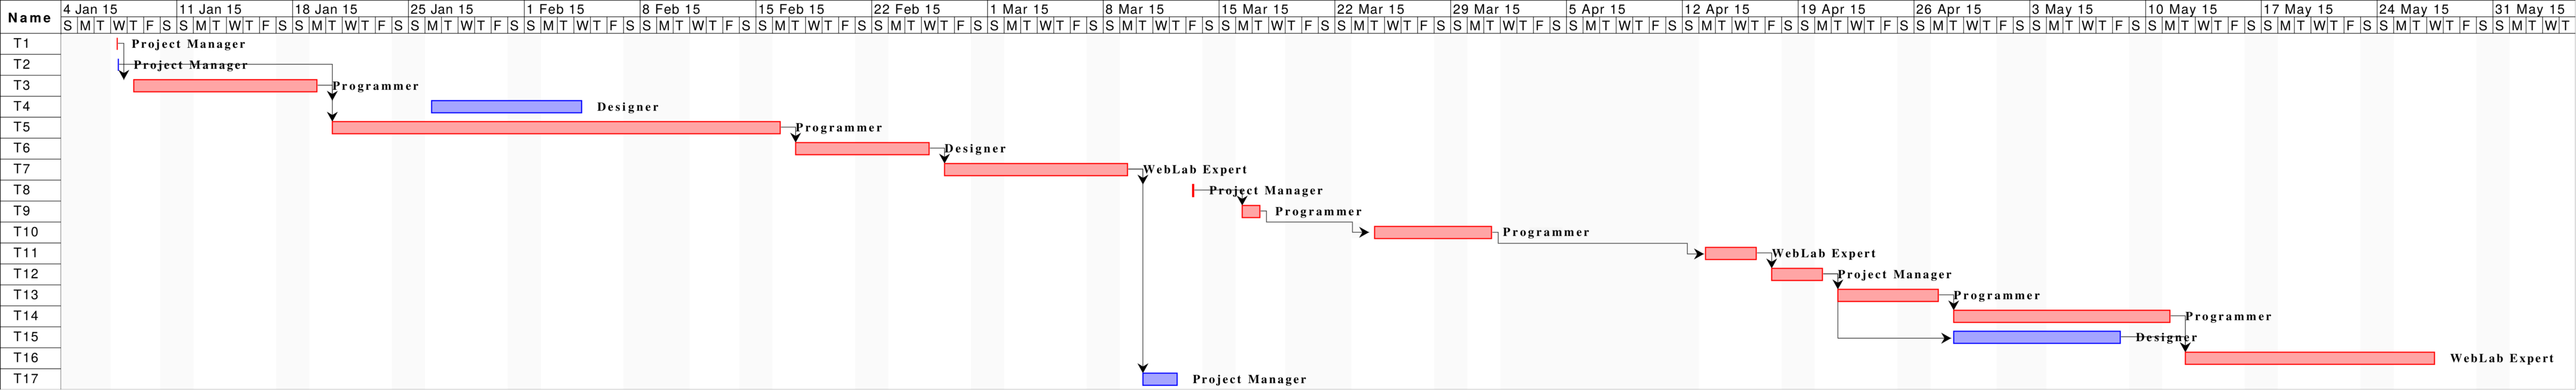
\includegraphics[trim=25.82in 0in 0in 0in, clip, angle=90]{fig/gantt}
\end{center}
\clearpage

% Precedence diagram in four pages
\clearpage
\begin{figure}
	\centering
	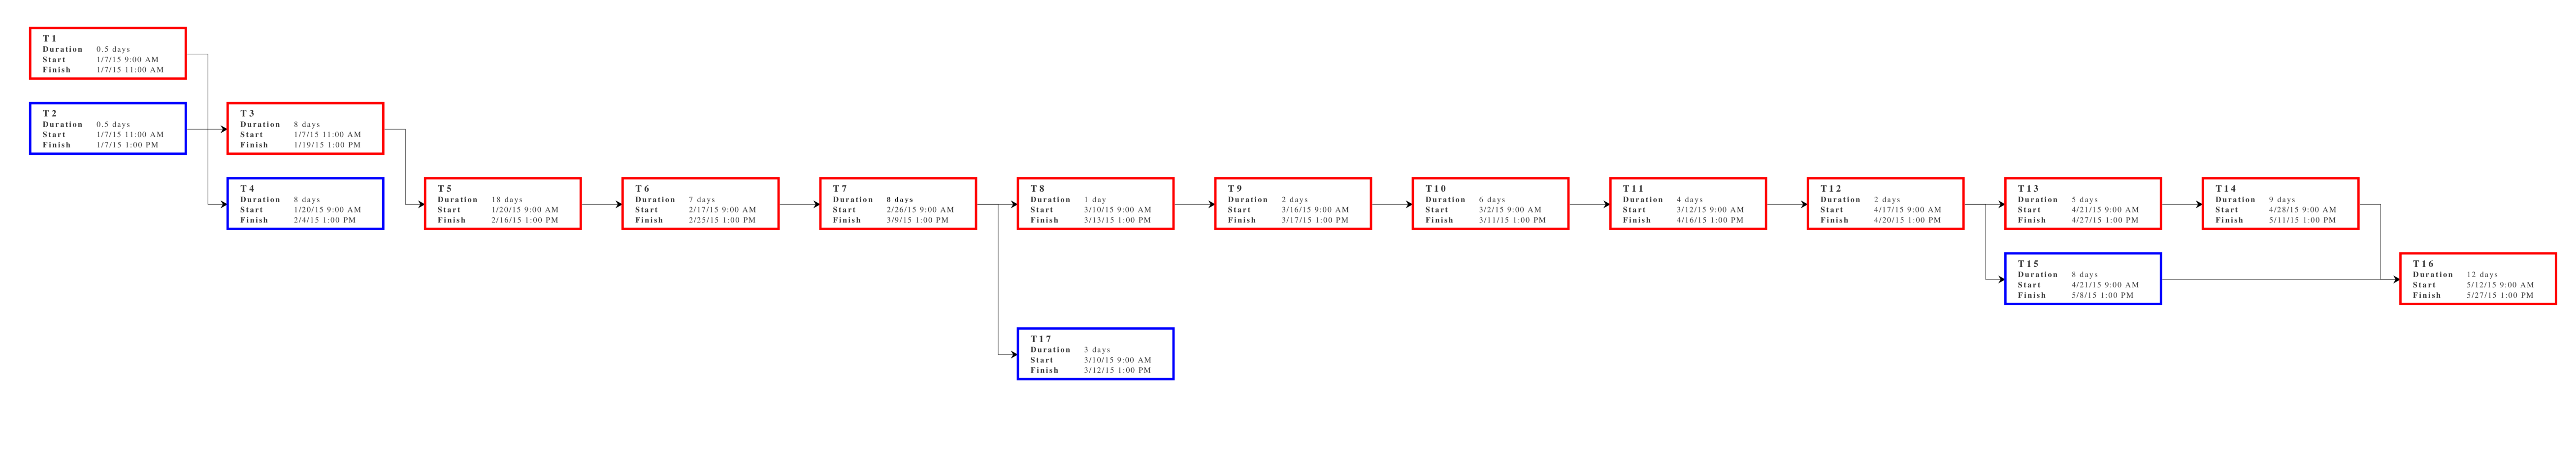
\includegraphics[trim=0in 0in 26in 0in, clip, angle=90]{fig/precedence}
	\caption[Precedence diagram of the project.]{Precedence diagram of the project. Continues in
	next pages.}\label{fig:precedence}
\end{figure}
\clearpage

\begin{center}
	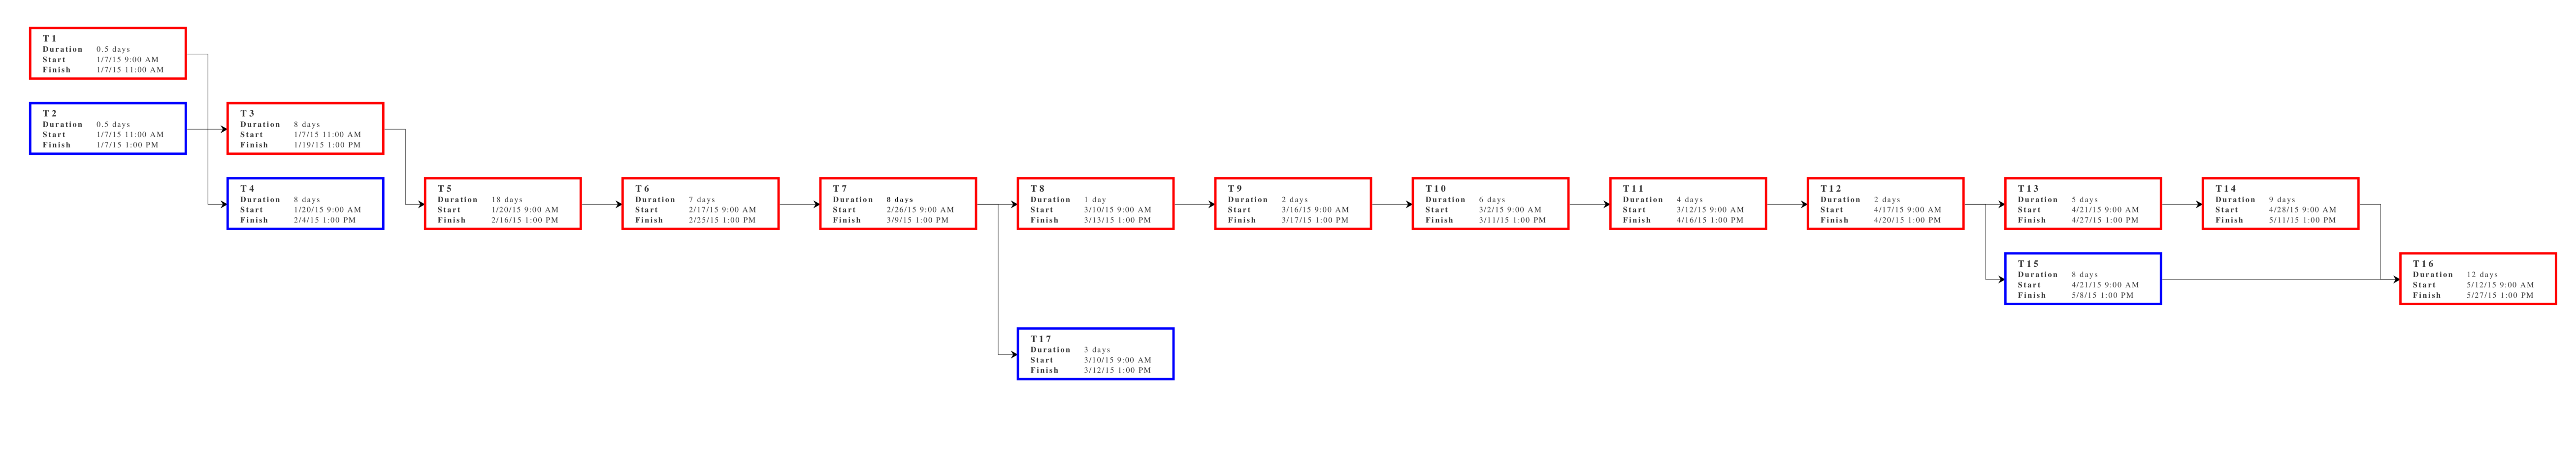
\includegraphics[trim=8.88in 0in 17in 0in, clip, angle=90]{fig/precedence}
	\clearpage

	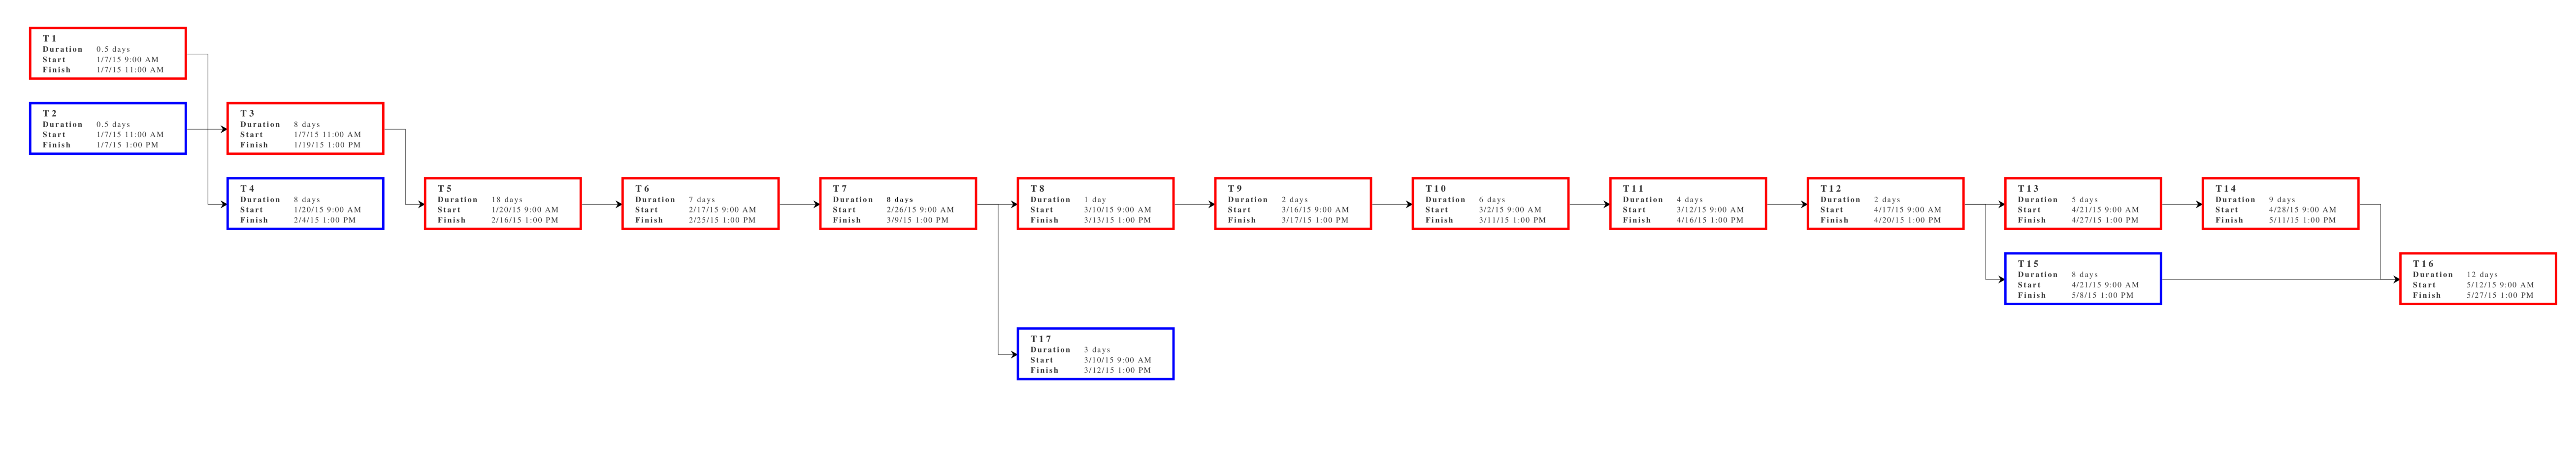
\includegraphics[trim=17.88in 0in 8in 0in, clip, angle=90]{fig/precedence}
	\clearpage

	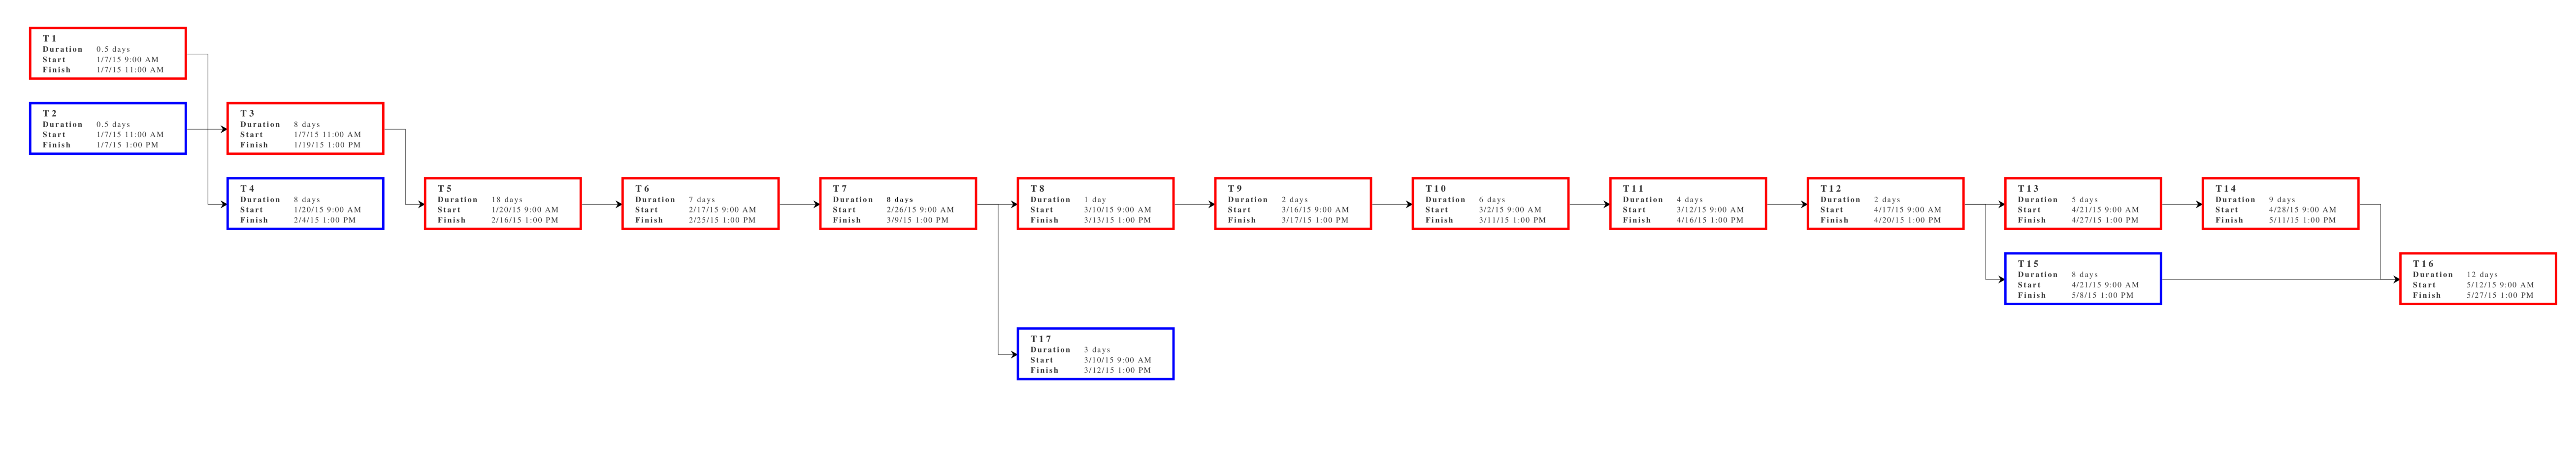
\includegraphics[trim=26.88in 0in 0in 0in, clip, angle=90]{fig/precedence}
\end{center}
\clearpage
